\documentclass[11pt,a4paper]{article}
\usepackage[top=2.5cm, bottom=2cm, left=2cm, right=2cm]{geometry}
\usepackage{amsmath}
\usepackage{tikz}
\usepackage{circuitikz}
\usepackage{epigraph}
\usepackage{hyperref}
\usepackage{multirow}
%\usepackage[demo]{graphicx}
\usepackage{caption}
\usepackage{subcaption}
\setcounter{secnumdepth}{5}
\usepackage{chngcntr}
\counterwithin{figure}{section}
\counterwithin{table}{section}
\counterwithin{equation}{section}
\usepackage{multirow}
\setcounter{tocdepth}{5}
\usepackage{subfiles}

\renewcommand\epigraphflush{flushright}
\renewcommand\epigraphsize{\normalsize}
\setlength\epigraphwidth{0.7\textwidth}

\usepackage{color}
\definecolor{titlepagecolor}{cmyk}{1,.0,0.0,.50}
\definecolor{scolour}{cmyk}{1,.0,0.0,.85}
\definecolor{sscolour}{cmyk}{1,.0,0.0,.75}
\definecolor{ssscolour}{cmyk}{1,.0,0.0,.65}
\definecolor{paracolour}{cmyk}{1,.0,0.0,.55}

\usepackage{amsfonts}
%\DeclareFixedFont{\titlefont}{T1}{ams}{b}{sc}{0.5in}

% Added 
\usepackage{fancyhdr}
\pagestyle{fancy}
\lhead{MTRX3700 Jousting Robot}
\rhead{Faintree}
\cfoot{\thepage}
\renewcommand{\headrulewidth}{0.4pt}
\renewcommand{\footrulewidth}{0.4pt}
\renewcommand{\thepage}{\roman{page}}
\usepackage{indentfirst}           %remove if we dont want to indent
\renewcommand{\thepage}{\roman{page}}

\newcommand{\myparagraph}[1]{\paragraph{#1}\mbox{}\newline\indent}

\newlength{\normalparindent}
\AtBeginDocument{\setlength{\normalparindent}{\parindent}}

% Change heading colours
\usepackage{titlesec}
%\usepackage[usenames,dvipsnames]{xcolor}
\usepackage{bold-extra}
\titleformat{\section}
{\color{scolour}\scshape\huge\bfseries}
{\color{scolour}\thesection.}{2em}{}
\titleformat{\subsection}
{\color{sscolour}\normalfont\LARGE\bfseries}
{\color{sscolour}\thesubsection}{2em}{}
\titleformat{\subsubsection}
{\color{ssscolour}\normalfont\Large\bfseries}
{\hspace*{\normalparindent}\color{ssscolour}\thesubsubsection}{1em}{}
\titleformat{\paragraph}
{\color{paracolour}\normalfont\large\bfseries}
{\hspace*{\normalparindent}\color{paracolour}\theparagraph}{1em}{}

% end added
\makeatletter                       
\def\printauthor{%                  
    {\large \@author}}              
\makeatother
\author{%
    Lydia Drabsch \\
    311217591 \\
    \texttt{ldra3557@uni.sydney.edu.au}\vspace{20pt} \\
    Ayush Sharma \\
    311247431 \\
    \texttt{asha6047@uni.sydney.edu.au}\vspace{20pt} \\
    Leo Lou \\
    312078722\\
    \texttt{llou65587@uni.sydney.edu.au}\vspace{20pt}\\
    Bevan Jones \\
    312144881\\
    \texttt{bjon4634@uni.sydney.edu.au}\vspace{20pt}\\
    Ziji An \\
    312004966\\
    \texttt{zian5092@uni.sydney.edu.au}\vspace{20pt}\\
    Ziton Victor Zhang \\
    430415441\\
    \texttt{zzha1258@uni.sydney.edu.au}\\
    }


% Title image
\newcommand\titlepagedecoration{%
\tikz[remember picture,overlay] \node[opacity=1,inner sep=0pt] at ([xshift=5cm]current page.west){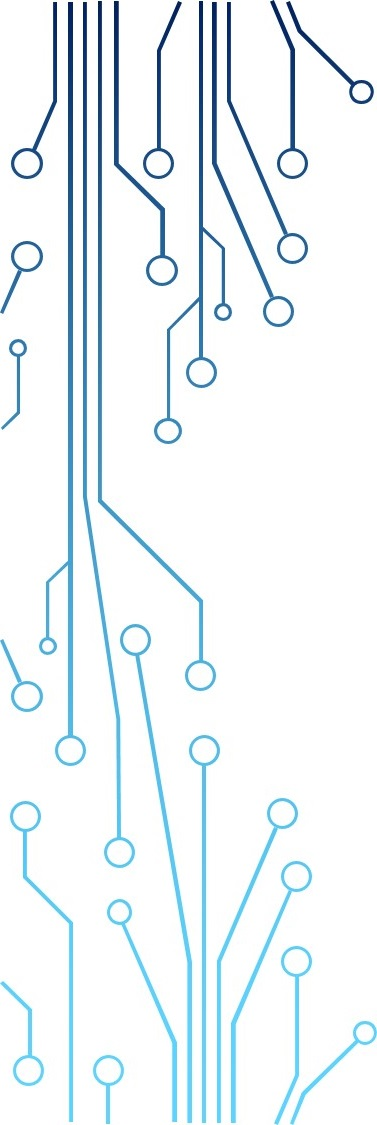
\includegraphics[height=\paperheight]{./IMAGEtitle2f}};
}

% added commands
\AtBeginDocument{\newcommand{\xd}{\dot{x} }}
\AtBeginDocument{\newcommand{\yd}{\dot{y} }}
\AtBeginDocument{\newcommand{\thetad}{\dot{\theta} }}
\AtBeginDocument{\newcommand{\cost}{\cos(\theta) }}
\AtBeginDocument{\newcommand{\sint}{\sin(\theta) }}
\AtBeginDocument{\newcommand{\xdd}{\ddot{x} }}
\AtBeginDocument{\newcommand{\ydd}{\ddot{y} }}
\AtBeginDocument{\newcommand{\thetadd}{\ddot{\theta} }}
\AtBeginDocument{\newcommand{\lam}{\vec{\lambda}}}
\usepackage{ amssymb }
\newcommand{\Lagr}{\mathcal{L}}
\usepackage{listings}
%\usepackage{float}
\AtBeginDocument{\newfloatcommand{capbtabbox}{table}[][\FBwidth]}
\usepackage{floatrow}

\begin{document}
\newgeometry{top=3.7cm, bottom=4cm, left=3cm, right=3cm}

\begin{titlepage}
\titlepagedecoration

\flushright
\huge{\scshape Technical Manual}\\ MTRX3700 Mechatronics 3 \\ Major Project 2015
\vfill
%\vspace{2cm}
\begin{minipage}{0.8\textwidth}
\centering
\rule{1\textwidth}{0.02pt}\\
\Huge{\textbf{\scshape Faintree}} \\
\huge{\scshape Charlemagne de la Robotic}
\\ \rule{1\textwidth}{0.02pt}\\
\end{minipage}
\vfill
%\null\vfill
%\vspace*{1cm}
%\noindent
%\hfill
\begin{minipage}{0.45\linewidth}
    \begin{flushright}
        \printauthor
    \end{flushright}
\end{minipage}
%
\begin{minipage}{0.02\linewidth}
    \rule{1pt}{370pt}
\end{minipage}


\end{titlepage}
\newgeometry{top=2.5cm, bottom=2cm, left=2cm, right=2cm}

%\begin{figure*}[h!]
%\centering
%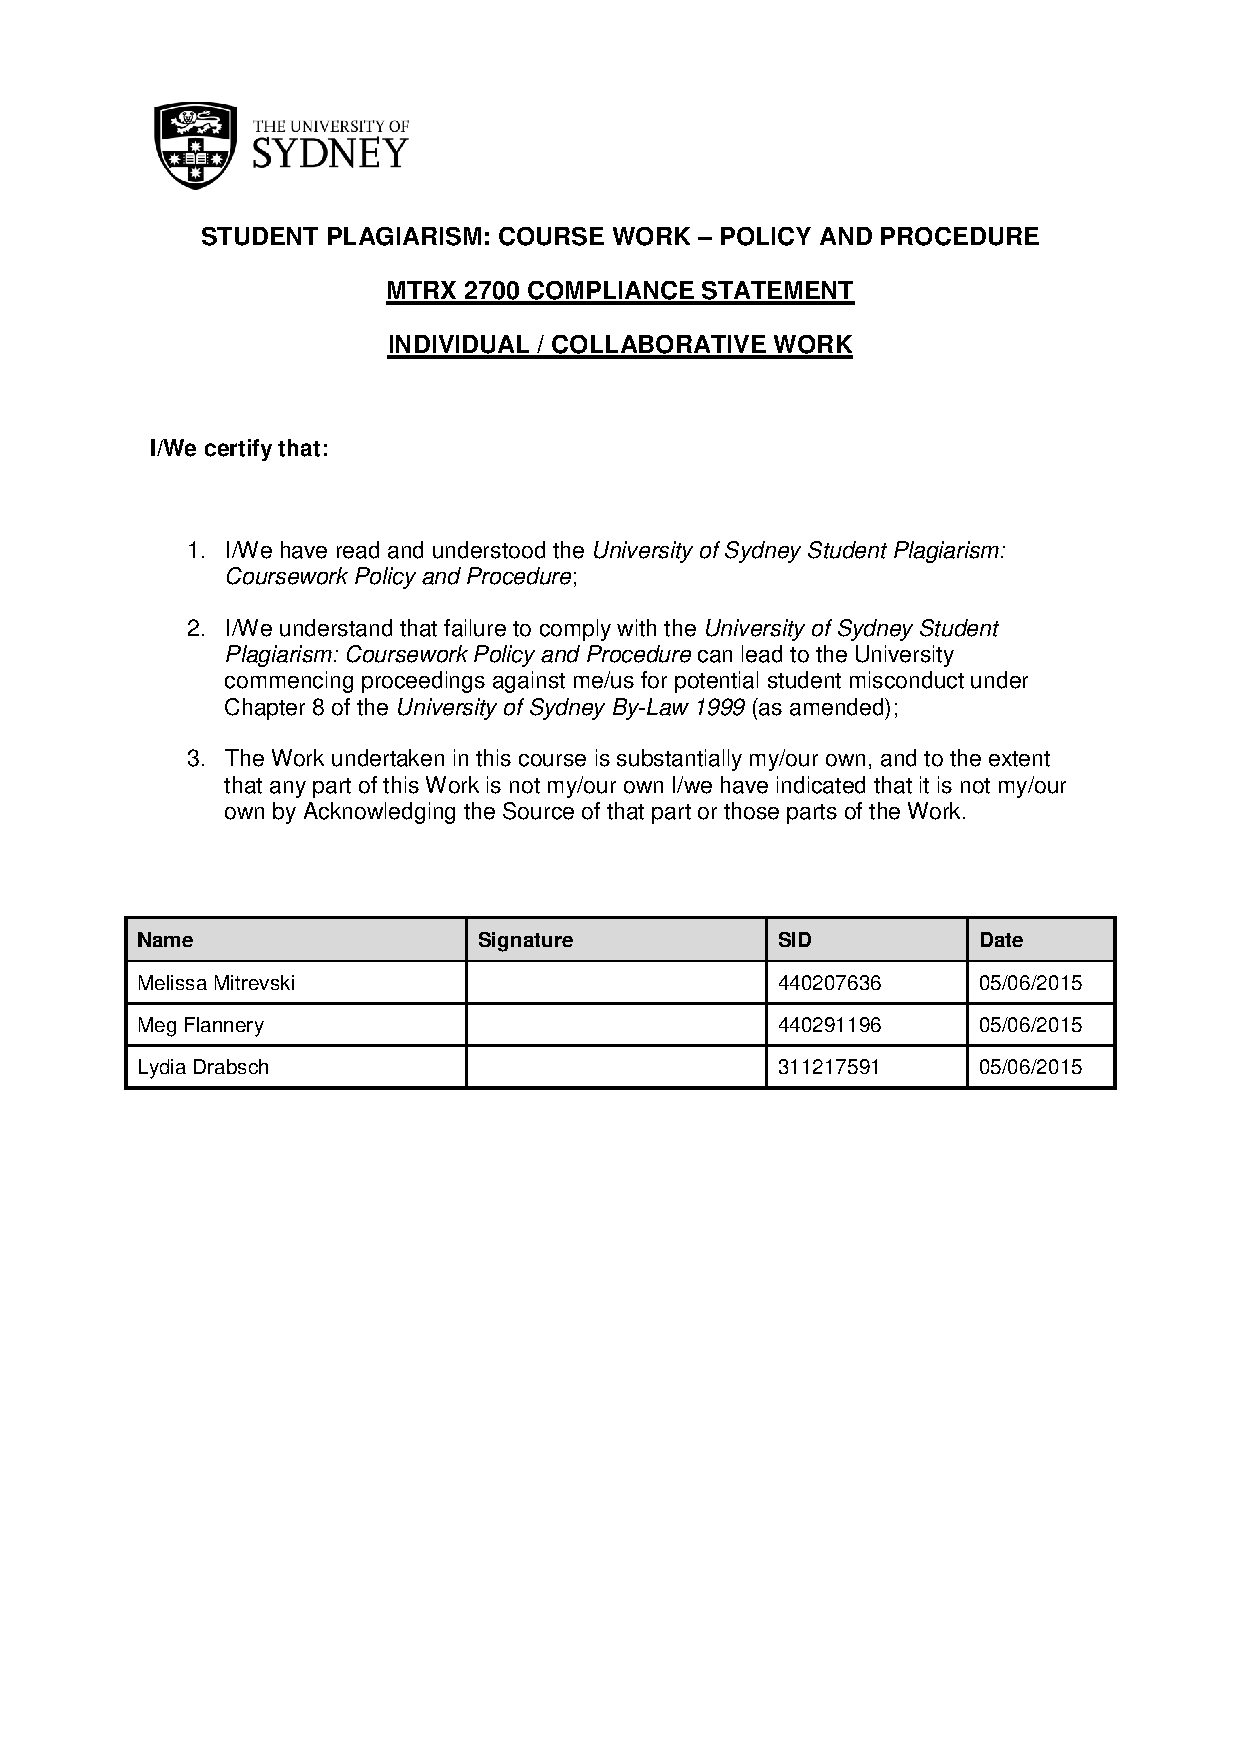
\includegraphics[width=0.99\linewidth]{./Plag}
%\label{fig:Plag}
%\end{figure*}

\setcounter{section}{0}



\tableofcontents
\listoffigures
\listoftables
\newpage
\pagenumbering{arabic}
%\renewcommand{\thepage}{\arabic{page}}


%\section{Introduction}
\subfile{Introduction}


%\section{System Description}
\subfile{System_Description}


% subsections
\subsection{Module Requirements: Menu Navigation}
\subfile{Menu_Nav} % leo

%\subfile{LCD} % leo

\subfile{Communications}  % ziji

\subfile{IRsensors}   % vic

\subfile{Manual_Mode}		      % Lydia

          % Lydia


% sections
\section{User Interface Design}
\subfile{User_Interface_Design}   % Leo

\section{Hardware Design}
\subfile{Hardware_Design}		  % Dpak

\section{Software Design}
\subfile{Software_Design}

\section{System Performance}
\subfile{System_Performance}
\subfile{Semiauto_Mode} 
\section{Safety Implications}
By law (NSW Occupational Health and Safety Act 2000; NSW Occupational Health and Safety
Regulation 2001) all employees who design plant, machinery or equipment must identify foreseeable safety hazards associated with the equipment, and then assess and control the identified risks. Although this law does not apply directly to student designs, you should consider it here.



\section{Conclusions}

\newpage
\bibliographystyle{IEEEtran}
\bibliography{file}


\newpage
\section{Appendix}

\end{document}